\documentclass[10pt,a4paper]{article}
\usepackage[utf8]{inputenc}
\usepackage[T1]{fontenc}
\usepackage{lmodern}
\usepackage{textcomp}
\renewcommand{\familydefault}{\sfdefault}
\usepackage[a4paper,left=2.1cm,right=2.1cm,top=2.2cm,bottom=2.4cm]{geometry}
\usepackage{amsmath}
\usepackage{amssymb}
\usepackage[table]{xcolor}
\usepackage{graphicx}
\usepackage{tabularx}
\usepackage{array}
\usepackage{enumitem}
\usepackage{titlesec}
\usepackage{needspace}
\usepackage{fancyhdr}
\usepackage[most]{tcolorbox}
\usepackage{tikz}
\usetikzlibrary{arrows.meta,positioning,calc}
\usepackage{xurl}
\usepackage{listings}
\usepackage[hidelinks]{hyperref}

% ------------------------------------------------------------- couleurs
\definecolor{secblue}{HTML}{2F5F8F}
\definecolor{subpurple}{HTML}{5A4FA6}
\definecolor{rulecol}{HTML}{C9D9EA}
\definecolor{fblue}{HTML}{DCE9F7}
\definecolor{fpurple}{HTML}{E6E3F5}
\definecolor{fgreen}{HTML}{DDF0E6}
\definecolor{fyellow}{HTML}{FCF2D3}
\definecolor{fpeach}{HTML}{FBE2D9}
\definecolor{fpink}{HTML}{F7DDE6}
\definecolor{fgray}{HTML}{EFEDEA}
\definecolor{rowgray}{HTML}{F2F1EE}
\definecolor{tgreen}{HTML}{2E7D5B}
\definecolor{tyellow}{HTML}{9A7414}
\definecolor{tpeach}{HTML}{B8573A}
\definecolor{tblue}{HTML}{2F5F8F}
\definecolor{tpurple}{HTML}{5A4FA6}
\definecolor{arrowcol}{HTML}{555555}

% ------------------------------------------------------------- mise en page
\setlength{\parindent}{0pt}
\setlength{\parskip}{0.45em}
\renewcommand{\arraystretch}{1.25}
\titleformat{\section}{\needspace{14\baselineskip}\Large\bfseries\color{secblue}}{\thesection.}{0.5em}{}[{\color{rulecol}\titlerule[0.8pt]}]
\titleformat{\subsection}{\needspace{8\baselineskip}\normalsize\bfseries\color{subpurple}}{\thesubsection}{0.6em}{}
\titlespacing*{\section}{0pt}{1.6em}{0.8em}
\titlespacing*{\subsection}{0pt}{1.2em}{0.5em}

\pagestyle{fancy}
\fancyhf{}
\renewcommand{\headrulewidth}{0pt}
\lfoot{\small Captain Energy -- Guide de la partie IA embarquée}
\rfoot{\small\thepage}

% boîte à titre en onglet : {fond}{couleur du titre}{titre}
\newtcolorbox{tbox}[3]{enhanced, colback=#1, colframe=#1,
  boxrule=0pt, arc=3mm, left=3mm, right=3mm, top=4.5mm, bottom=2mm,
  fonttitle=\bfseries\small, coltitle=#2, title={#3},
  attach boxed title to top left={xshift=3mm, yshift=-2.6mm},
  boxed title style={colback=white, colframe=#1!80!gray, boxrule=0.4pt, arc=2mm},
  before skip=4mm, after skip=3mm}

% pastille de numéro pour les étapes
\newcommand{\badge}[1]{{\setlength{\fboxsep}{2.2pt}\colorbox{fpurple}{\small\bfseries\color{secblue}#1}}}
\newlist{steps}{enumerate}{1}
\setlist[steps]{label=\badge{\arabic*}, leftmargin=1.9em, itemsep=0.35em}
\setlist[itemize]{itemsep=0.2em}

% figures reprises du document d'origine (vectorielles)



\newcolumntype{L}{>{\raggedright\arraybackslash}X}
\newcolumntype{P}[1]{>{\raggedright\arraybackslash}p{#1}}
\newcolumntype{Q}[1]{>{\raggedright\arraybackslash\bfseries}p{#1}}

\definecolor{codebg}{HTML}{F6F5F2}
\lstdefinestyle{code}{basicstyle=\ttfamily\scriptsize, backgroundcolor=\color{codebg}, frame=single, rulecolor=\color{codebg},
  numbers=left, numberstyle=\tiny\color{gray}, numbersep=6pt, xleftmargin=1.8em, breaklines=true, columns=fullflexible, keepspaces=true,
  commentstyle=\color{tgreen}, keywordstyle=\color{secblue}\bfseries, showstringspaces=false, aboveskip=0.6em, belowskip=0.6em,
  literate={é}{{\'e}}1 {è}{{\`e}}1 {à}{{\`a}}1 {ç}{{\c c}}1 {ê}{{\^e}}1 {°}{{\textdegree}}1 {ù}{{\`u}}1 {î}{{\^i}}1 {ô}{{\^o}}1
           {É}{{\'E}}1 {µ}{{$\mu$}}1 {«}{{\guillemotleft}}1 {»}{{\guillemotright}}1 {â}{{\^a}}1 {û}{{\^u}}1 {ï}{{\"i}}1 {À}{{\`A}}1 {È}{{\`E}}1 {Ê}{{\^E}}1 {ç}{{\c c}}1}
\lstdefinestyle{cmd}{style=code, numbers=none, xleftmargin=0.5em, backgroundcolor=\color{fblue}, rulecolor=\color{fblue}, basicstyle=\ttfamily\footnotesize}
\lstset{style=code}
\newcommand{\code}[1]{\texttt{\small #1}}


\begin{document}

\begin{tcolorbox}[enhanced, colback=fblue, colframe=fblue, arc=4mm, boxrule=0pt, left=5mm, right=5mm, top=4mm, bottom=4mm]
{\fontsize{22}{26}\selectfont\bfseries\color{secblue} Captain Energy -- Guide de la partie IA embarquée}\par\vspace{2mm}
{\large\color{subpurple} Edge Energy Manager -- le problème, le matériel, le câblage, les trois IA, les résultats}\par\vspace{2mm}
{\small\color{gray!70!black} TSYP14 Technical Challenge «~Edge AI \& IoT for Resilient Smart Infrastructure~» -- maquette : ESP32, 2 packs 3S 18650, 2 INA219, 2 DS18B20, Peltier TEC1-12704 sur relais}
\end{tcolorbox}

\begin{tbox}{fpurple}{tpurple}{Ce que vous allez construire}
Toute l'intelligence tourne \textbf{sur l'ESP32}, sans Internet. Elle est faite de quatre blocs~:
\begin{enumerate}[nosep, leftmargin=2em]
  \item \textbf{IA n°1 -- état du réseau~:} un petit réseau de neurones (poids en int8) reconnaît chaque seconde si la tension STEG (mesurée par l'INA219) est \emph{normale}, \emph{instable}, \emph{en baisse} ou \emph{coupée}.
  \item \textbf{IA n°2 -- batterie~:} niveau de charge et autonomie, avec la tension et le courant \textbf{mesurés} par l'INA219 n°2.
  \item \textbf{IA n°3 -- temps de sécurité~:} l'ESP32 apprend tout seul la vitesse de réchauffement $k$ de la boîte (2 DS18B20~: air du frigo et magasin), puis un \textbf{réseau entraîné sur 40\,000 coupures simulées} donne, dès la première seconde de la coupure, combien de temps la marchandise reste sûre. Il n'y a pas de sonde dans la marchandise~: $T_{\text{produit}}$ est une \textbf{donnée simulée}.
  \item \textbf{Score de risque + moteur de décision~:} prévoit la coupure, \textbf{pré-refroidit vraiment} avec le Peltier, décide quels appareils (LED) garder et envoie les alertes.
\end{enumerate}
Le PC ne sert qu'à \textbf{entraîner} les modèles n°1 et n°3 (une fois) et, en bonus, à envoyer les \textbf{annonces STEG et la météo}.
\end{tbox}

% =====================================================================
\section{Le problème et notre réponse}\label{sec:probleme}

\subsection{Le problème}
En été, le réseau STEG est très chargé (climatiseurs, chaleur). Les petits commerces avec un frigo (épiceries, boucheries, laiteries, pharmacies) subissent alors trois choses~:
\begin{itemize}
  \item \textbf{des baisses de tension et un réseau instable}~: la tension descend ou oscille sans couper complètement~;
  \item \textbf{des retours de courant rapides}~: le courant revient, recoupe, revient en quelques minutes. Le compresseur du frigo redémarre alors sous pression, tire un très fort courant de démarrage, chauffe et finit par griller~;
  \item \textbf{des coupures longues}~: le frigo s'arrête, la marchandise se réchauffe sans que personne ne le sache. Le commerçant jette la marchandise, ou pire, la vend alors qu'elle n'est plus sûre (viande, lait, insuline et vaccins entre 2 et 8~°C).
\end{itemize}
\textbf{Ce qui existe ne suffit pas~:} un \textbf{protège-tension} coupe le courant quand la tension est mauvaise et attend avant de rallumer, mais il n'a pas de batterie~; un \textbf{onduleur} (UPS) alimente \emph{tout} jusqu'à se vider, sans priorité. Aucun des deux ne sait \textbf{combien de temps la marchandise reste sûre}, ni ne prépare le frigo avant la coupure.

{\small\textit{Pour le rapport~: citez des chiffres vérifiés (coupures STEG des étés récents, nombre de commerces, pertes de la chaîne du froid) avec leur source primaire et leur année. Ce guide ne donne volontairement aucun chiffre non vérifié.}}

\subsection{Notre réponse : Captain Energy}
Un boîtier placé entre la STEG, une batterie et les appareils du commerce. Il \textbf{décide sur place}, avec trois petites IA qui tournent sur l'ESP32~:
\begin{enumerate}[nosep, leftmargin=2em]
  \item \textbf{avant la coupure}~: il reconnaît un réseau qui se dégrade (IA n°1), calcule un score de risque et \textbf{pré-refroidit} le frigo pour stocker du froid~;
  \item \textbf{pendant la coupure}~: il passe sur batterie, calcule l'\textbf{autonomie} (IA n°2) et le \textbf{temps de sécurité} de la marchandise (IA n°3), garde le frigo en priorité, coupe le reste, et prévient «~vendez avant HH:MM~» si la batterie ne suffira pas~;
  \item \textbf{au retour}~: il attend un réseau stable et rallume les appareils un par un, avec un délai pour le compresseur.
\end{enumerate}

\subsection{La chaîne demandée par le cahier des charges}
\rowcolors{2}{white}{rowgray}
\begin{tabularx}{\linewidth}{P{3.2cm}L}
\rowcolor{fblue} \textbf{Maillon} & Dans Captain Energy \\
Sensing (capteurs) & 2 INA219 (tension STEG~; tension et courant de la batterie), 2 DS18B20 (air du frigo, air du magasin) \\
Edge processing & ESP32~: IA n°1 (état du réseau), IA n°2 (batterie), IA n°3 (temps de sécurité), score de risque, moteur de décision, détection de porte. \textbf{Tout est calculé sur place, sans cloud.} \\
Connectivity & Wi-Fi + MQTT~: annonces de coupure STEG et météo reçues, alertes envoyées (téléphone via ntfy), commandes à distance \\
Response / Action & Relais du Peltier (froid, pré-refroidissement), délestage des appareils (LED clim et lumières), LED de couleur, buzzer, écran OLED, alertes \\
\end{tabularx}
\textbf{Sans Internet, le boîtier fonctionne quand même}~: Internet n'ajoute que les annonces, la météo et les alertes téléphone.

% =====================================================================
\section{Avant de commencer : les priorités}\label{sec:prio}

La Phase 1 se rend le \textbf{20/11}. Faites les étapes dans cet ordre~: chacune donne déjà une démo qui marche.

\rowcolors{2}{white}{rowgray}
\begin{tabularx}{\linewidth}{P{1.2cm}LP{3.2cm}}
\rowcolor{fpeach} Ordre & \mdseries Étape & \mdseries Pour \\
1 & Installer VS Code et PlatformIO, câbler, régler \code{config.h}, téléverser le firmware principal avec le modèle de test fourni (sections \ref{sec:avoir} à \ref{sec:fichiers} et \ref{sec:miseenroute}). & Vidéo du 20/11 \\
2 & Collecter vos mesures de tension et entraîner le vrai modèle n°1 (section \ref{sec:ia1}, environ 1 h 30). & Vidéo du 20/11 \\
3 & Refroidir la boîte, puis \code{pause=45} pour que l'ESP32 apprenne $k$ (section \ref{sec:ia3}). & Vidéo du 20/11 \\
4 & Tourner la démo avec les commandes série (section \ref{sec:demo}). & Vidéo du 20/11 \\
5 & Mosquitto + script des annonces STEG et de la météo + alertes sur téléphone (section \ref{sec:risque}). & Finale \\
6 & Mesurer temps d'inférence, mémoire, précision réelle~; graphique de $k$ pour le rapport. & Rapport et finale \\
\end{tabularx}

\begin{tbox}{fpeach}{tpeach}{Important : le modèle fourni est un modèle de test}
Le fichier \code{grid\_model.h} livré a été entraîné sur des \textbf{données synthétiques}, juste pour vérifier que toute la chaîne fonctionne. Ses 99,5~\% ne valent rien pour le jury. Remplacez-le par un modèle entraîné sur \textbf{vos} mesures (section \ref{sec:ia1}), et donnez la précision \textbf{réelle}, même si elle est plus basse.
\end{tbox}

% =====================================================================
\section{Le matériel utilisé}\label{sec:avoir}

\subsection{Les composants de la maquette}
\rowcolors{2}{white}{rowgray}
\begin{tabularx}{\linewidth}{P{4.6cm}P{0.7cm}LP{2.1cm}}
\rowcolor{fgreen} Composant & \mdseries Qté & \mdseries Rôle dans la maquette & \mdseries Broches \\
ESP32 DevKit V1 + câble USB (données) & 1 & Le cerveau~: mesures, trois IA, décisions. \textbf{Alimenté par l'USB du PC}, pour rester allumé quand on coupe la «~STEG~» & USB \\
INA219 n°1 (adresse 0x40) & 1 & Tension de la «~STEG~», 100 fois par seconde (IA n°1) & I2C 21 / 22 \\
INA219 n°2 (0x41, pont A0 soudé) & 1 & Tension et courant du pack n°2 (IA n°2, protections du Peltier) & I2C 21 / 22 \\
\textbf{Pack n°1}~: 3 cellules 18650 (3,7 V, 1500 mAh) en série + potentiomètre 10 k$\Omega$ & 1 & Simule la STEG~: tourner = baisse ou instabilité, débrancher = coupure. Seulement mesuré & -- \\
\textbf{Pack n°2}~: 3 cellules 18650 (3,7 V, 1500 mAh) en série, soit 11,1 V et 1,5 Ah & 1 & Batterie de secours~: alimente le Peltier et le ventilateur & -- \\
Fusible rapide 5 A + porte-fusible & 1 & Protège le pack n°2 contre un court-circuit & -- \\
Peltier \textbf{TEC1-12704} + 2 dissipateurs + ventilateur 12 V + pâte thermique & 1 & Le «~moteur du frigo~»~: froid réel (environ 3 A) & -- \\
Module relais 2 canaux 5 V (JQC-3FF-S-Z, 10 A, commande à l'état bas) & 1 & Canal 1, contact NO~: allume et éteint le Peltier & IN1 = GPIO18 \\
Sonde DS18B20 étanche & 2 & Air dans le frigo~; air du magasin ($T_{\text{amb}}$) & GPIO4 \\
Résistance 4,7 k$\Omega$ & 1 & Rappel du fil de données des DS18B20 vers 3,3 V & GPIO4 \\
Boîte en polystyrène (+ bouteille d'eau, optionnel) & 1 & Le «~frigo~» (et une masse froide, comme une marchandise) & -- \\
LED + résistance 220 $\Omega$ & 2 & Simulent le climatiseur et les lumières (délestage) & 25, 33 \\
LED RGB (cathode commune) + 3 $\times$ 220 $\Omega$ & 1 & Vert = normal, orange = batterie, rouge = danger & 16, 17, 23 \\
Buzzer actif 3--5 V & 1 & Un son différent par situation & 19 \\
Écran OLED 0,96'' I2C (SSD1306, 0x3C) & 1 & Autonomie, temps de sécurité, alertes & I2C 21 / 22 \\
Plaque d'essai, fils Dupont, fils 0,75 mm² et borniers à vis & -- & Signaux sur la plaque~; \textbf{courant du Peltier par fils épais et borniers, jamais par la plaque} & -- \\
Multimètre & 1 & Vérifier les tensions, la continuité, le contact du relais & -- \\
\end{tabularx}

{\small Ce qui n'est \textbf{pas} sur la maquette (version produit)~: sonde dans la marchandise, comparateur LM393 (coupure matérielle), MOSFET de démarrage doux, carte KiCad, boîtier rail DIN, module vocal DFPlayer Mini, lecteur RFID RC522.}

\subsection{Les logiciels utilisés}
\rowcolors{2}{white}{rowgray}
\begin{tabularx}{\linewidth}{P{4.6cm}L}
\rowcolor{fgreen} Logiciel & \mdseries Pour quoi \\
VS Code + extension \textbf{PlatformIO IDE} & Écrire, compiler et téléverser le firmware de l'ESP32 (framework Arduino) \\
Bibliothèques ESP32 (installées par PlatformIO) & Adafruit INA219, OneWire, DallasTemperature, Adafruit SSD1306 + GFX, PubSubClient (MQTT), ArduinoJson \\
Python 3 + extension Python de VS Code & Collecte des données et entraînement des modèles (\code{tools/}) \\
Paquets Python & pyserial (port série), numpy, pandas, scikit-learn (réseaux de neurones), matplotlib (graphiques), requests et paho-mqtt (annonces, météo, alertes) \\
Mosquitto & Serveur MQTT sur le PC (annonces STEG, météo, alertes) \\
ntfy (application téléphone) & Recevoir les alertes sur le téléphone \\
Open-Meteo & Prévisions de température (gratuit, sans clé) \\
g++ & Tester la logique du firmware sur PC (\code{tests/}) \\
\end{tabularx}

\textbf{Pourquoi deux packs~?} Pour simuler une coupure, on débranche le pack n°1 («~STEG~»)~; le pack n°2 continue d'alimenter le Peltier, comme une vraie batterie de secours. Avec un seul pack, la tension mesurée chuterait à chaque démarrage du Peltier, et l'IA n°1 croirait à une baisse du réseau. Le niveau du pack n°2 est \textbf{calculé} à partir de sa tension et du courant mesurés par l'INA219 n°2 (section \ref{sec:ia2}).

% =====================================================================
\section{Ce qu'il faut installer (VS Code)}\label{sec:install}

\subsection{VS Code et ses extensions}
\begin{steps}
  \item Installer \textbf{VS Code} (code.visualstudio.com) et \textbf{Python 3.11 ou 3.12} (python.org~; sous Windows, cocher «~Add Python to PATH~»). PlatformIO a besoin de Python.
  \item Dans VS Code, ouvrir l'onglet \textbf{Extensions} (Ctrl+Maj+X) et installer~:
\end{steps}

\rowcolors{2}{white}{rowgray}
\begin{tabularx}{\linewidth}{P{4.6cm}P{1.9cm}L}
\rowcolor{fblue} \textbf{Extension} & Obligatoire & Pour \\
PlatformIO IDE \textit{(PlatformIO)} & oui & Compiler, téléverser sur l'ESP32, moniteur série, bibliothèques automatiques \\
Python \textit{(Microsoft)} & oui & Lancer les scripts d'entraînement et de collecte \\
Pylance \textit{(Microsoft)} & conseillé & Autocomplétion et erreurs dans le code Python \\
C/C++ \textit{(Microsoft)} & installée avec PlatformIO & Autocomplétion dans le code ESP32 \\
Rainbow CSV & facultatif & Lire les fichiers de mesures CSV en couleur \\
\end{tabularx}

Le projet contient un fichier \code{.vscode/extensions.json}~: en ouvrant le dossier, VS Code \textbf{propose lui-même} d'installer ces extensions.

\begin{steps}[resume]
  \item Après l'installation de PlatformIO, \textbf{redémarrer VS Code}. Une icône de fourmi apparaît dans la barre de gauche~: PlatformIO télécharge ses outils la première fois (quelques minutes).
  \item Brancher l'ESP32. S'il n'est pas reconnu, installer le pilote USB de la puce écrite sur la carte~: \textbf{CP210x} ou \textbf{CH340}.
\end{steps}

\textbf{Pas besoin d'installer les bibliothèques à la main~:} elles sont listées dans \code{platformio.ini} et PlatformIO les télécharge à la première compilation (INA219, OneWire, DallasTemperature, OLED, MQTT, JSON).

\subsection{Python dans VS Code (environnement virtuel)}
Un environnement virtuel garde les paquets du projet à part. Dans le terminal de VS Code (Ctrl+ù ou \textbf{Terminal $\rightarrow$ Nouveau terminal}), depuis le dossier \code{tools}~:
\begin{lstlisting}[style=cmd]
python -m venv .venv
.venv\Scripts\activate          (Windows)      source .venv/bin/activate   (Linux, Mac)
pip install -r requirements.txt
\end{lstlisting}
Puis Ctrl+Maj+P $\rightarrow$ \textbf{Python: Select Interpreter} $\rightarrow$ choisir \code{.venv}. Si Windows refuse d'activer l'environnement, taper une fois \code{Set-ExecutionPolicy -Scope CurrentUser RemoteSigned} dans PowerShell.

\subsection{Mosquitto et ntfy (finale seulement)}
\textbf{Mosquitto} (mosquitto.org) relie le PC, l'ESP32 et le téléphone. Depuis la version 2, il faut un fichier \code{mosquitto.conf} avec ces deux lignes, puis lancer \code{mosquitto -c mosquitto.conf -v}~:
\begin{lstlisting}[style=cmd]
listener 1883 0.0.0.0
allow_anonymous true
\end{lstlisting}
\textbf{ntfy} (application gratuite)~: abonnez-vous à un sujet difficile à deviner, par exemple \code{eem-cold-7f3k}, pour recevoir les alertes.

% =====================================================================
\section{Le câblage}\label{sec:cablage}

\subsection{Les signaux vers l'ESP32}
\rowcolors{2}{white}{rowgray}
\begin{tabularx}{\linewidth}{P{4.2cm}LP{2.2cm}}
\rowcolor{fblue} \textbf{Composant} & Branchement & ESP32 \\
Alimentation de l'ESP32 & \textbf{Câble USB du PC} (5 V). Jamais par le pack n°1~: l'ESP32 s'éteindrait pendant la coupure qu'il doit gérer & USB \\
INA219 n°1, INA219 n°2 et OLED (même bus I2C) & SDA / SCL / VCC / GND, en parallèle & 21 / 22 / 3V3 / GND \\
2 DS18B20 (même fil) & Rouge $\rightarrow$ 3V3, noir $\rightarrow$ GND, jaune (DATA) des deux sondes ensemble $\rightarrow$ GPIO4~; \textbf{4,7 k$\Omega$ entre DATA et 3V3} & GPIO4 \\
Adresse de l'INA219 n°2 & \textbf{Souder le pont A0} (deux petites pastilles marquées A0) & 0x41 \\
Module relais (côté broches) & VCC $\rightarrow$ 5 V (VIN)~; GND~; \textbf{IN1} $\rightarrow$ GPIO18~; cavalier JD-VCC en place & GPIO18 \\
LED clim / lumières & GPIO $\rightarrow$ 220 $\Omega$ $\rightarrow$ LED $\rightarrow$ GND & 25 / 33 \\
LED RGB (R / V / B), buzzer & Même montage~; buzzer + sur la broche & 16 / 17 / 23, 19 \\
\end{tabularx}

{\small Les DS18B20 partagent un seul fil~: chaque sonde a une adresse unique. Sans la 4,7 k$\Omega$, l'ESP32 lit $-127$~°C. Les deux INA219 sortent d'usine à la même adresse (0x40)~: \textbf{sans le pont A0 sur le n°2, l'ESP32 ne peut pas les distinguer}.}

\subsection{La partie puissance}
\begin{lstlisting}[style=cmd]
"STEG"     : pack n°1 (+) -> potentiomètre (patte du bout) ; autre patte -> pack n°1 (-) / GND
             patte du milieu du potentiomètre -> INA219 VIN+   (VIN- non branché)
"Batterie" : pack n°2 (+) -> fusible 5 A -> INA219 n°2 -> COM1 du relais
             (avant cela : fusible -> INA219 n°2 VIN+ ; VIN- -> COM1)
             NO1 du relais -> Peltier (+)
             Peltier (-) -> pack n°2 (-)
             Ventilateur : sur le pack n°2 APRÈS le fusible mais AVANT l'INA219 n°2
             (toujours allumé ; son courant n'est pas compté dans celui du Peltier)
Masses communes : pack n°1 (-), pack n°2 (-), ESP32 GND
\end{lstlisting}
Utilisez le contact \textbf{NO1} (normalement ouvert)~: si l'ESP32 est éteint ou redémarre, le Peltier reste éteint. Le module relais est commandé à l'état bas (\code{RELAY\_ACTIVE\_LOW 1}).

\textbf{Si le relais reste collé ou claque mal~:} problème connu de ces modules avec la logique 3,3 V de l'ESP32. Retirez le cavalier JD-VCC, branchez \textbf{JD-VCC sur 5 V} (bobines) et \textbf{VCC sur 3,3 V} (optocoupleurs), GND commun.

\begin{tbox}{fpeach}{tpeach}{Protéger le Peltier et les composants}
\begin{itemize}[nosep]
  \item \textbf{Jamais de Peltier sans dissipateur et ventilateur côté chaud}, même 2 secondes~: il se détruit et peut brûler. Pâte thermique des deux côtés, dissipateur bien serré. Ventilateur branché \textbf{directement} sur le pack n°2, toujours allumé.
  \item \textbf{Fusible 5 A} sur le + du pack n°2, au plus près des cellules. Le TEC1-12704 tire environ 3 à 3,5 A~; le fusible coupe en cas de court-circuit, même si l'ESP32 est planté.
  \item \textbf{Fils épais} (au moins 0,75 mm²) et \textbf{borniers à vis} pour le Peltier~: \textbf{jamais par la plaque d'essai}, qui chauffe au-delà de 1 à 2 A.
  \item \textbf{Relais~:} contacts 10 A / 30 V continu, largement suffisants. Le firmware laisse au moins 3 minutes entre deux démarrages, ce qui ménage aussi le relais.
  \item \textbf{Cellules Li-ion~:} touchez-les après 5 minutes~; si elles chauffent, arrêtez. Rechargez avant que le pack descende à 9 V (3 V par cellule)~: l'INA219 n°2 mesure le pack et alerte sous 9,6 V. Jamais de court-circuit entre + et $-$.
  \item \textbf{INA219~:} 26 V maximum, et environ \textbf{3,2 A} maximum avec sa résistance de mesure de 0,1 $\Omega$. Le TEC1-12704 tire environ 3 A, juste à la limite~: au-delà, la mesure plafonne (sans danger pour le module à ce courant), donc la protection logicielle contre la surintensité ne voit plus rien et \textbf{le fusible reste indispensable}. Jamais de tension de pack sur une broche de l'ESP32.
  \item \textbf{Protections du programme} (section \ref{sec:ia2})~: coupure immédiate au-dessus de 5 A et alerte si le Peltier ne consomme rien. Elles complètent le fusible, elles ne le remplacent pas.
  \item \textbf{Avant chaque mise sous tension~:} vérifier au multimètre les tensions et l'absence de court-circuit, Peltier débranché, puis brancher le Peltier en dernier.
\end{itemize}
\end{tbox}

\subsection{Le «~frigo~» de la maquette}
\begin{steps}
  \item Monter le Peltier dans le couvercle de la boîte en polystyrène~: face froide (avec un petit dissipateur) dedans, face chaude (grand dissipateur + ventilateur) dehors.
  \item Fixer la sonde DS18B20 «~air~» à l'intérieur, au milieu, sans toucher le dissipateur froid.
  \item Poser la sonde DS18B20 «~magasin~» dehors, à l'ombre, loin du ventilateur chaud.
  \item Optionnel~: une bouteille d'eau dans la boîte. Elle n'a pas de sonde ($T_{\text{produit}}$ reste simulée), mais elle ajoute de la masse froide, comme une vraie marchandise.
\end{steps}

% =====================================================================
\section{Les fichiers du projet et VS Code}\label{sec:fichiers}

\subsection{L'organisation}
\begin{lstlisting}[style=cmd]
edge_energy_manager.code-workspace   à ouvrir dans VS Code (tout le projet d'un coup)
.vscode/extensions.json              extensions proposées automatiquement
firmware/collect_grid/               projet PlatformIO de collecte (IA n°1, étape 1)
    platformio.ini                   carte + bibliothèques
    src/main.cpp                     mesure la tension, envoie les caractéristiques
firmware/edge_energy_manager/        projet PlatformIO principal du boîtier
    platformio.ini                   carte + bibliothèques + moniteur série
    src/main.cpp                     capteurs, machine à états, Peltier, LED, écran, MQTT
    src/config.h                     TOUS vos réglages (Wi-Fi, broches, capteurs, seuils)
    src/grid_features.h              IA n°1 : les 8 caractéristiques d'une fenêtre
    src/tinyml.h                     IA n°1 : le réseau de neurones int8
    src/grid_model.h                 IA n°1 : les poids (généré par Python)
    src/battery.h                    IA n°2 : niveau de charge et autonomie
    src/thermal.h                    IA n°3 : apprentissage de k, formule de Newton
    src/safety_model.h               IA n°3 : poids du réseau du temps de sécurité (généré par Python)
    src/safety_ai.h                  IA n°3 : le réseau, exécuté sur l'ESP32
    src/door_detect.h                porte ouverte déduite des températures (pas de contact)
    src/decision.h                   score de risque + moteur de décision + profils
tools/                               scripts Python (PC), dont train_safety_model.py (IA n°3)
tests/                               tests de la logique sur PC
\end{lstlisting}

Les fichiers \code{.h} de l'IA n'utilisent aucune fonction Arduino~: ils ont été \textbf{compilés et testés sur PC} (section \ref{sec:tests}). Le \code{main.cpp} a été compilé avec des bibliothèques simulées~; il n'a pas encore tourné sur une vraie carte, donc vérifiez-le pas à pas (section \ref{sec:miseenroute}).

\subsection{Les gestes de base dans VS Code}
\begin{steps}
  \item \textbf{Fichier $\rightarrow$ Ouvrir l'espace de travail à partir d'un fichier} $\rightarrow$ \code{edge\_energy\_manager.code-workspace}. Les deux projets PlatformIO, les outils et les tests apparaissent dans l'explorateur.
  \item En bas de la fenêtre, la \textbf{barre bleue de PlatformIO}~: \textbf{$\checkmark$} compiler (Build), \textbf{$\rightarrow$} téléverser (Upload), \textbf{prise} moniteur série (Serial Monitor), \textbf{poubelle} nettoyer (Clean). Un sélecteur indique le \textbf{projet actif}~: choisissez \code{env:esp32dev (Firmware principal)} ou \code{(Collecte)} avant de cliquer.
  \item La première compilation télécharge la plateforme ESP32 et les bibliothèques~: comptez plusieurs minutes, ensuite c'est rapide.
  \item \textbf{Moniteur série~:} tapez une commande (\code{info}, \code{pause=60}\ldots) puis \textbf{Entrée}~: elle est envoyée à l'ESP32 (réglé dans \code{platformio.ini} avec \code{send\_on\_enter}).
  \item \textbf{Un seul programme à la fois} peut utiliser le port USB~: fermez le moniteur série (Ctrl+C dans son terminal, ou la poubelle du terminal) avant de lancer \code{log\_serial.py} ou \code{thermal\_log.py}, et avant de téléverser.
  \item Si le téléversement échoue avec «~Failed to connect~», maintenez le bouton \textbf{BOOT} de l'ESP32 quand «~Connecting...~» s'affiche.
\end{steps}

\subsection{Ce que vous devez modifier dans le code, étape par étape}
Vous n'avez \textbf{presque rien à programmer}~: la logique est écrite et testée. Votre travail dans le code, c'est de \textbf{régler} le projet pour votre matériel.

\textbf{Étape A -- \code{firmware/edge\_energy\_manager/src/config.h}}

\rowcolors{2}{white}{rowgray}
\begin{tabularx}{\linewidth}{P{4.4cm}P{2.6cm}L}
\rowcolor{fgreen} \textbf{Réglage} & Valeur & Ce que vous devez faire \\
\code{WIFI\_SSID}, \code{WIFI\_PASS} & votre Wi-Fi & Le partage de connexion d'un téléphone suffit. \code{""} pour travailler sans Wi-Fi. \\
\code{MQTT\_HOST} & IP du PC & Seulement avec Mosquitto~: \code{ipconfig} (Windows) donne l'adresse IPv4. \\
\code{TEMP\_SENSOR\_DHT11} & 0 & Vous utilisez des DS18B20. \\
\code{IDX\_AIR}, \code{IDX\_AMB} & 0, 1 & Ordre des sondes sur le fil~: à inverser si l'ESP32 confond le frigo et le magasin. \\
\code{HAS\_PRODUCT\_PROBE} & 0 & Pas de sonde dans la marchandise~: $T_{\text{produit}}$ est simulée. \\
\code{PROD\_TAU\_MIN} & 15 & Retard de la $T_{\text{produit}}$ simulée sur l'air (plus grand = produit plus «~lourd~»). \\
\code{SAFETY\_USE\_AI} & 1 & Temps de sécurité par le réseau appris (0 = formule de Newton seule). \\
\code{HAS\_DOOR\_SWITCH} & 0 & Pas de contact de porte~: l'ouverture est déduite des températures. \\
\code{DOOR\_RISE\_C} & 0.30 & Montée de l'air en 10 s qui signifie «~porte ouverte~» (à régler, section \ref{sec:porte}). \\
\code{HAS\_BATTERY\_INA}, \code{CURRENT\_FROM\_INA2} & 1, 1 & L'INA219 n°2 mesure la tension et le courant du pack n°2. \\
\code{HAS\_CURRENT\_SENSOR} & 0 & Pas d'ACS712 (mettre 1 seulement si vous en ajoutez un). \\
\code{BAT\_EMPTY\_V} & 9.6 & Sous cette tension, batterie considérée vide et alerte. \\
\code{REAL\_COOLING} & 1 & Le Peltier refroidit vraiment. \\
\code{PELTIER\_USE\_RELAY} & 1 & Peltier commandé par le module relais (marche / arrêt). \\
\code{RELAY\_ACTIVE\_LOW} & 1 & Votre module s'active à l'état bas. Mettre 0 si le Peltier s'allume au démarrage. \\
\code{SUPPLY\_V} & 11.1 & Tension du pack n°2, pour calculer la puissance du Peltier. \\
\code{PELTIER\_MAX\_A}, \code{PELTIER\_MIN\_A} & 5.0, 0.3 & Limites de courant du TEC1-12704 (coupure / alerte). \\
\code{BAT\_CAPACITY\_AH} & 1.5 & Capacité du pack n°2~: 3 cellules 18650 de 1500 mAh en série. \\
\code{PIN\_LED\_ROUTER} & -1 & Pas de LED routeur dans votre maquette. \\
\code{STABLE\_S}, \code{COMP\_MIN\_OFF\_S} & 120, 180 & Peuvent être réduits pour une vidéo courte (en le disant). \\
\code{DEMO\_SPEED} & 1 & 30 pour voir la batterie se vider en quelques minutes. \\
\code{DEFAULT\_PROFILE} & \code{PROF\_MAQUETTE} & Profil au démarrage. \\
\end{tabularx}

\textbf{Étape B -- \code{src/decision.h}, ligne du profil «~maquette~».} Après un premier essai, regardez la température la plus basse que votre boîte atteint (par exemple 11~°C), et réglez $T_{\min}$ juste au-dessus et $T_{\max}$ 5 à 6~°C plus haut~: \code{\{"maquette", 12.0f, 17.0f\}}.

\textbf{Étape C -- \code{src/grid\_model.h} et \code{src/safety\_model.h}.} Ne les modifiez pas à la main~: \code{train\_grid\_model.py} et \code{train\_safety\_model.py} les réécrivent (sections \ref{sec:ia1} et \ref{sec:ia3}).

\textbf{Étape D -- \code{tools/outage\_feed.py} (finale).} Vérifiez les adresses \code{FEEDS} et lancez le script avec votre zone (\code{-{}-zone}).

\textbf{Après chaque modification~:} \textbf{$\checkmark$} pour compiler, puis \textbf{$\rightarrow$} pour téléverser.

% =====================================================================
\section{IA n°1 : reconnaître l'état du réseau}\label{sec:ia1}

\subsection{Le principe}
L'ESP32 mesure la tension 100 fois par seconde. Chaque seconde, il résume la fenêtre en \textbf{8 nombres}, puis un petit réseau de neurones dit à quelle classe cette seconde ressemble.

\rowcolors{2}{white}{rowgray}
\begin{tabularx}{\linewidth}{P{0.9cm}P{4.4cm}L}
\rowcolor{fpurple} \textbf{N°} & Caractéristique & Ce qu'elle révèle \\
f0 & Moyenne & Le niveau de tension \\
f1, f2 & Minimum, maximum & Les creux et les pics \\
f3 & Écart-type & Une tension qui bouge beaucoup (instable) \\
f4 & Pente (V/s) & Une tension qui descend lentement (baisse) \\
f5 & Part du temps sous 10,4 V & Une sous-tension \\
f6 & Part du temps sous 1 V & Une coupure \\
f7 & Variation moyenne entre deux mesures & Des oscillations rapides \\
\end{tabularx}

Avec 8 nombres au lieu de 100 mesures, le réseau est minuscule (192 poids), s'entraîne avec peu de données et tourne en quelques dizaines de microsecondes.

\subsection{Étape 1 : téléverser le programme de collecte}
Dans la barre PlatformIO, choisir le projet \textbf{Collecte}, puis \textbf{$\rightarrow$} (Upload). Ouvrir le moniteur série (\textbf{prise})~: une ligne \code{F,...} doit apparaître chaque seconde. \textbf{Fermez ensuite le moniteur}~: le script Python a besoin du port. Les commandes ci-dessous se tapent dans le terminal de VS Code, dans le dossier \code{tools}, environnement \code{.venv} activé.

\subsection{Étape 2 : enregistrer les quatre situations}
Remplacez \code{COM5} par votre port (PlatformIO l'affiche pendant le téléversement~; sous Linux \code{/dev/ttyUSB0})~:
\begin{lstlisting}[style=cmd]
python log_serial.py --port COM5 --label normal   --seconds 180 --out data/normal.csv
python log_serial.py --port COM5 --label baisse   --seconds 180 --out data/baisse.csv
python log_serial.py --port COM5 --label instable --seconds 180 --out data/instable.csv
python log_serial.py --port COM5 --label coupure  --seconds 120 --out data/coupure.csv
\end{lstlisting}

\rowcolors{2}{white}{rowgray}
\begin{tabularx}{\linewidth}{P{1.8cm}L}
\rowcolor{fyellow} \textbf{Classe} & Ce que vous faites avec le potentiomètre du pack n°1 («~STEG~») \\
normal & Rester entre 11,0 et 11,7 V (votre batterie «~STEG~»). Tourner un peu le potentiomètre de temps en temps. \\
baisse & Descendre \textbf{lentement} de 11,5 V à 10 V~; rester entre 10 et 10,8 V~; recommencer. \\
instable & Tourner le potentiomètre \textbf{vite}, d'avant en arrière, entre 10,6 et 11,7 V~; débrancher un fil moins d'une demi-seconde, plusieurs fois. \\
coupure & Fil de la patte du milieu débranché de VIN+. Le débrancher et le rebrancher quelques fois au début. \\
\end{tabularx}

Faites deux séances par classe à des moments différents (les données s'ajoutent au même fichier). Visez au moins 150 fenêtres par classe.

\subsection{Étape 3 : entraîner et exporter}
\begin{lstlisting}[style=cmd]
python train_grid_model.py data/normal.csv data/baisse.csv data/instable.csv data/coupure.csv
\end{lstlisting}
\begin{steps}
  \item Il met de côté \textbf{25~\%} des fenêtres pour le test~: le modèle ne les voit jamais pendant l'apprentissage.
  \item Il \textbf{normalise} chaque caractéristique (moyenne 0, écart-type 1).
  \item Il entraîne un réseau \textbf{8 $\rightarrow$ 16 (ReLU) $\rightarrow$ 4}.
  \item Il \textbf{quantifie} les poids en int8~: une échelle par couche $s = \max|W| / 127$, chaque poids devient un entier entre $-127$ et $127$.
  \item Il donne la précision \textbf{avant et après} quantification et la \textbf{matrice de confusion}.
  \item Il écrit \code{grid\_model.h} directement dans le dossier du firmware principal.
\end{steps}
Une confusion entre \emph{baisse} et \emph{normal} vers 11--11,5 V est normale (cas limites). Si une classe est mal reconnue, enregistrez plus de données pour elle. Recopiez la précision int8 et la matrice dans le rapport.

\subsection{Le réseau sur l'ESP32, ligne par ligne}
\lstinputlisting[language=C++, firstline=20, lastline=54, firstnumber=20]{../firmware/edge_energy_manager/src/tinyml.h}
\begin{itemize}
  \item \textbf{Ligne 25~:} normalisation avec la moyenne et l'écart-type de l'entraînement~; sans elle, le modèle reçoit des nombres à la mauvaise échelle.
  \item \textbf{Lignes 28--33~:} couche cachée. Somme «~poids int8 $\times$ entrée~», puis on multiplie \textbf{une seule fois} par l'échelle \code{GM\_S1} et on ajoute le biais. \code{ReLU} remplace les valeurs négatives par 0.
  \item \textbf{Lignes 36--40~:} couche de sortie, 4 scores (un par classe).
  \item \textbf{Lignes 43--52~:} softmax~: les scores deviennent des probabilités (total 100~\%), on garde la plus grande. On soustrait le maximum (ligne 47) pour éviter un dépassement dans \code{expf}.
\end{itemize}
\textbf{Ce qui est en int8~:} les \textbf{poids} (192 octets au lieu de 768)~; les calculs se font en float, très rapides sur l'ESP32. Au jury~: «~poids quantifiés en int8~».

\subsection{Comment le firmware l'utilise}
\lstinputlisting[language=C++, firstline=331, lastline=348, firstnumber=331]{../firmware/edge_energy_manager/src/main.cpp}
\begin{itemize}
  \item \textbf{Lignes 332--334~:} une mesure toutes les 10 ms~; après un retard (écran, Wi-Fi), on repart proprement.
  \item \textbf{Lignes 336--339~:} la tension est rangée dans la fenêtre de 100 mesures.
  \item \textbf{Lignes 341--345~:} caractéristiques, réseau, et \textbf{temps d'inférence} (\code{inferUs}) à donner au jury.
  \item \textbf{Ligne 346~:} moyenne glissante de «~instable ou baisse~», qui alimente le score de risque.
  \item \textbf{Ligne 347~:} trois secondes de «~baisse~» sûre à plus de 85~\% font passer sur batterie \textbf{avant} la coupure. Les seuils fixes (10,4 V et 13,3 V) restent actifs~: l'IA anticipe, les règles protègent.
\end{itemize}

% =====================================================================
\section{IA n°3 : le temps de sécurité de la marchandise}\label{sec:ia3}

\subsection{Le principe}
L'IA n°3 répond à une seule question, \textbf{dès la première seconde de la coupure}~: \emph{combien de temps la marchandise reste-t-elle sûre si le froid s'arrête~?} C'est ce \textbf{temps de sécurité} qui commande toutes les décisions (section \ref{sec:decision}).

Elle a deux parties~:
\begin{enumerate}[nosep, leftmargin=2em]
  \item \textbf{Apprentissage de $k$ sur place}~: quand le Peltier est éteint, la boîte se réchauffe selon la loi de Newton $\frac{dT}{dt} = k\,(T_{\text{amb}} - T)$. L'ESP32 mesure la vitesse de montée et l'écart avec le magasin, et en déduit $k$ (la «~vitesse de réchauffement~» de \emph{votre} frigo).
  \item \textbf{Un réseau de neurones entraîné sur 40\,000 coupures simulées}, qui donne le temps de sécurité à partir de $T_{\text{produit}}$, $T_{\text{air}}$, $T_{\text{amb}}$, $T_{\max}$, $k$ et des ouvertures de porte.
\end{enumerate}

\subsection{Les températures : 2 sondes réelles, 1 simulée}
\rowcolors{2}{white}{rowgray}
\begin{tabularx}{\linewidth}{P{2.6cm}P{3.6cm}L}
\rowcolor{fblue} \textbf{Grandeur} & D'où elle vient & Rôle \\
$T_{\text{air}}$ & DS18B20 n°1, dans le frigo & Réagit vite (saute quand la porte s'ouvre) \\
$T_{\text{amb}}$ & DS18B20 n°2, dans le magasin & Ce qui réchauffe le frigo \\
$T_{\text{produit}}$ & \textbf{simulée} (fausse donnée) & Ce qui compte pour la sécurité~: la marchandise \\
$T_{\max}$ & profil choisi (\code{decision.h}) & Limite de la marchandise (4~°C volaille, 8~°C médicaments, 16~°C maquette) \\
\end{tabularx}

Il n'y a pas de sonde dans la marchandise. Dans le boîtier, $T_{\text{produit}}$ est donc fabriquée à partir de l'air~: un produit suit l'air avec retard, à cause de sa masse (filtre du premier ordre, $\tau = 15$~min, \code{PROD\_TAU\_MIN})~:
\[ T_{\text{produit}} \leftarrow T_{\text{produit}} + \frac{\Delta t}{\tau}\,(T_{\text{air}} - T_{\text{produit}}) \]
\lstinputlisting[language=C++, firstline=434, lastline=449, firstnumber=434]{../firmware/edge_energy_manager/src/main.cpp}
\begin{itemize}
  \item \textbf{Lignes 434--438~:} lecture des deux DS18B20 par leur adresse~; $-127$ veut dire «~sonde absente~», on garde l'ancienne valeur.
  \item \textbf{Lignes 439--441~:} si un jour vous ajoutez une 3e sonde dans le produit (\code{HAS\_PRODUCT\_PROBE 1}), elle remplace la valeur simulée.
  \item \textbf{Lignes 444--447~:} sinon, la valeur simulée rattrape l'air d'un petit pas toutes les 2 s. Porte ouverte, elle ne suit pas~: l'air chaud qui entre quelques secondes ne réchauffe presque pas la marchandise.
\end{itemize}

\subsection{Le jeu de données : toutes les coupures possibles}
Pour \textbf{entraîner} le réseau, il faut des milliers de coupures dont on connaît la vraie réponse. On ne peut pas couper un vrai frigo 40\,000 fois~: le script \code{tools/train\_safety\_model.py} les \textbf{simule}. Pour chaque coupure, il tire au hasard une situation, puis simule pas à pas (toutes les 10 s) l'air et la marchandise, moteur éteint, jusqu'à ce que la marchandise dépasse $T_{\max}$. Le temps obtenu est la \textbf{vraie} réponse.

\rowcolors{2}{white}{rowgray}
\begin{tabularx}{\linewidth}{P{4.2cm}L}
\rowcolor{fgreen} \textbf{Ce qui varie} & Plage couverte \\
Type de frigo & Petite boîte Peltier (comme la maquette) ou vrai frigo de commerce (vide à plein, bien ou mal isolé) \\
$T_{\max}$ & 4, 8, 10 ou 16~°C (les profils) dans 70~\% des cas, sinon n'importe quelle valeur de 2 à 18~°C \\
$T_{\text{produit}}$ au début & de 10~°C sous $T_{\max}$ jusqu'à juste en dessous~; 5~\% des cas déjà au-dessus (réponse 0) \\
$T_{\text{air}}$ au début & de 3~°C sous le produit à 2~°C au-dessus (moteur qui vient de tourner, ou porte qui vient de s'ouvrir) \\
$T_{\text{amb}}$ & 18 à 42~°C, qui peut monter jusqu'à +3~°C/h pendant la coupure (après-midi d'été) \\
Ouvertures de porte & 0 à 20 par heure, 5 à 60 s chacune, à des moments au hasard \\
$k$ & calculé à partir de l'isolation et de la masse, avec $\pm 20$~\% d'erreur (comme le $k$ appris sur place) \\
\end{tabularx}

Le jeu complet est écrit dans \code{tools/safety\_dataset.csv} (40\,000 lignes, utile pour le rapport). 80~\% servent à l'entraînement, 20~\% au test sur des coupures jamais vues.

\subsection{Le réseau et ses entrées}
7 entrées $\rightarrow$ 16 neurones (ReLU) $\rightarrow$ 1 sortie, poids en \textbf{int8} (129 octets de poids). Les entrées sont les 6 grandeurs du tableau, plus le résultat de la \textbf{formule de Newton} (en logarithme)~: le réseau part de la physique et apprend à la corriger (portes, air plus chaud que le produit, magasin qui se réchauffe). Il sort $\log(t + 0{,}05)$~: une erreur de 6 minutes compte autant sur 30 minutes que 2 heures sur 10 heures.

\begin{lstlisting}[style=cmd]
cd tools
python train_safety_model.py --plot      (environ 1 minute)
\end{lstlisting}
Le script réécrit \code{src/safety\_model.h} et \code{tools/safety\_model\_testvectors.csv}, puis affiche~:

\rowcolors{2}{white}{rowgray}
\begin{tabularx}{\linewidth}{P{4.6cm}P{2.8cm}L}
\rowcolor{fpeach} \textbf{Méthode (8\,000 coupures de test)} & Erreur relative médiane & Surestime de plus de 10~\% \\
Formule de Newton seule (avant) & 33~\% & 25,6~\% des cas \\
Réseau int8 (sur l'ESP32) & \textbf{23~\%} & 38,9~\% des cas \\
Réseau int8 $\times$ marge 0,51 (\textbf{utilisé}) & 50~\% & \textbf{3,3~\%} des cas \\
\end{tabularx}

\textbf{Pourquoi une marge~?} Surestimer le temps de sécurité est dangereux (on laisse le moteur éteint trop longtemps)~; le sous-estimer coûte seulement un peu de batterie. Le script calcule le facteur \code{SM\_MARGIN} qui rend 95~\% des prédictions prudentes. Le réseau est plus juste que Newton~; avec la marge, il est \textbf{beaucoup plus prudent} (3~\% de cas trop optimistes au lieu de 26~\%).

\begin{center}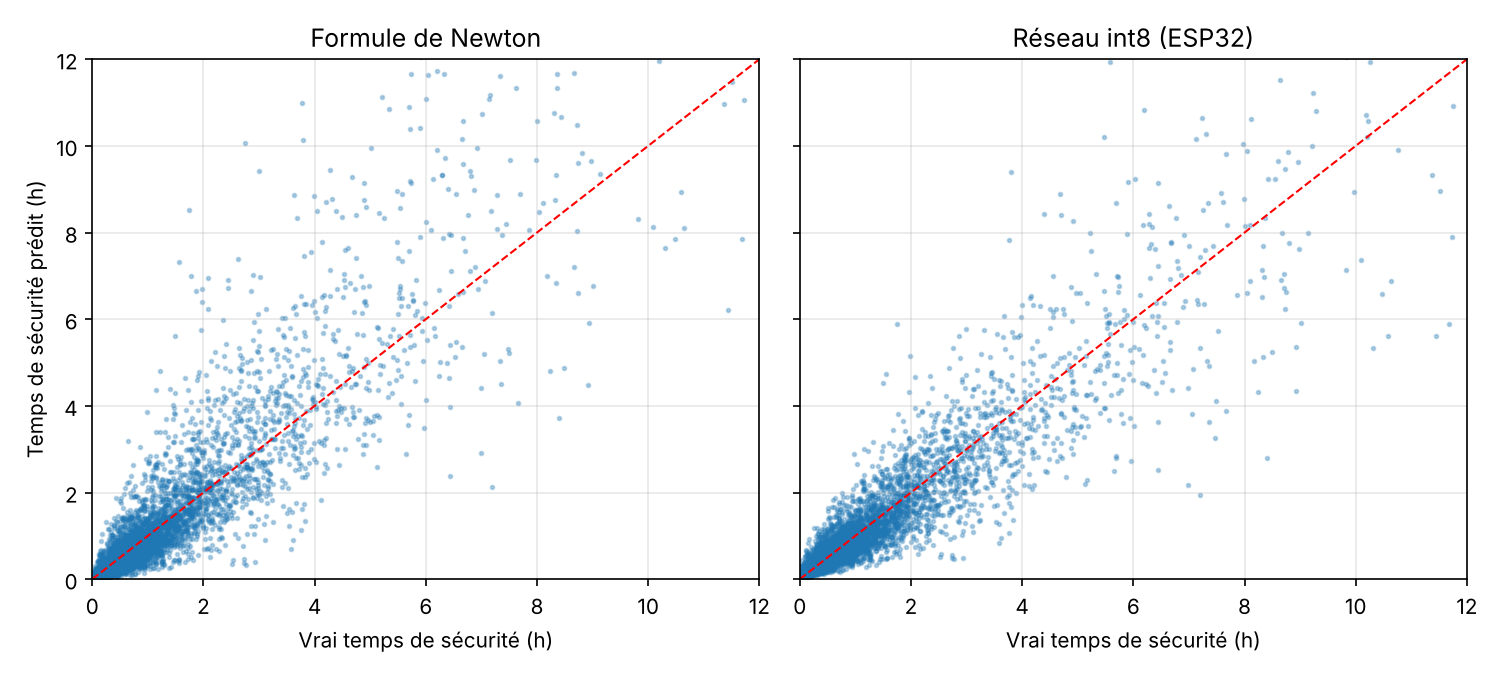
\includegraphics[width=0.92\linewidth]{temps_securite_test.png}\end{center}
{\small Chaque point est une coupure de test~: vrai temps (horizontal) contre temps prédit (vertical). Sur la diagonale rouge, la prédiction est parfaite.}

\textbf{Pourquoi l'erreur ne descend pas à 0~:} au début de la coupure, personne ne sait quand la porte sera ouverte ni de combien le magasin va se réchauffer. Cette part du hasard ne peut pas être devinée~; c'est pour cela que la marge existe.

\subsection{Le réseau sur l'ESP32, ligne par ligne}
\lstinputlisting[language=C++, firstline=9, lastline=35, firstnumber=9]{../firmware/edge_energy_manager/src/safety_ai.h}
\begin{itemize}
  \item \textbf{Lignes 10--15~:} formule de Newton, exactement comme dans Python (7e entrée). Magasin plus froid que $T_{\max}$~: jamais dangereux (99 h).
  \item \textbf{Lignes 20--23~:} les 7 entrées, normalisées avec la moyenne et l'écart-type du jeu d'entraînement.
  \item \textbf{Lignes 24--30~:} couche cachée~: somme des poids int8 $\times$ entrées, mise à l'échelle (\code{SM\_S1}), biais, ReLU~; puis la sortie.
  \item \textbf{Lignes 31--34~:} retour de $\log(t+0{,}05)$ à des heures, borné entre 0 et 24 h.
\end{itemize}
Dans \code{decision.h}, le temps retenu est \code{safeTimeAI(...) * SM\_MARGIN}~; avec \code{SAFETY\_USE\_AI 0}, on revient à la formule de Newton seule.

\subsection{Les DS18B20 et la pente de température}
Le DS18B20 mesure au 0,0625~°C près. Le firmware calcule la pente par \textbf{régression linéaire} sur une fenêtre de \textbf{5 minutes} (6 mesures, une par minute), ce qui lisse le bruit~:
\lstinputlisting[language=C++, firstline=46, lastline=57, firstnumber=46]{../firmware/edge_energy_manager/src/thermal.h}
\begin{itemize}
  \item \textbf{Lignes 47--49~:} moyenne du temps et des températures de la fenêtre.
  \item \textbf{Lignes 51--55~:} pente des moindres carrés~: tous les points comptent.
  \item \textbf{Ligne 56~:} on passe de °C par minute à °C par heure.
\end{itemize}
Le code garde aussi le mode DHT11 (\code{TEMP\_SENSOR\_DHT11 1}, fenêtre de 30 minutes), testé avec des mesures arrondies au degré.

\subsection{L'apprentissage, ligne par ligne}
\lstinputlisting[language=C++, firstline=63, lastline=86, firstnumber=63]{../firmware/edge_energy_manager/src/thermal.h}
\begin{itemize}
  \item \textbf{Lignes 64--67~:} on garde les dernières mesures (une par minute)~; rien n'est appris avant que la fenêtre soit pleine (5 minutes).
  \item \textbf{Lignes 69--73~:} pente de la fenêtre et écart moyen avec le magasin.
  \item \textbf{Ligne 75~:} on n'apprend que si c'est permis (Peltier éteint et porte fermée pendant toute la fenêtre), si l'écart dépasse 2~°C et si la température monte.
  \item \textbf{Lignes 77--79~:} moindres carrés avec oubli ($\lambda = 0{,}98$)~: deux nombres en mémoire suffisent, et $k$ s'adapte si on remplit ou vide la boîte.
  \item \textbf{Lignes 83--85~:} Peltier allumé pendant toute la fenêtre~: on apprend aussi la \textbf{vitesse de refroidissement}, qui sert à calculer quand commencer le pré-refroidissement.
\end{itemize}

La formule de Newton (utilisée comme entrée du réseau, et seule si \code{SAFETY\_USE\_AI 0})~:
\lstinputlisting[language=C++, firstline=88, lastline=94, firstnumber=88]{../firmware/edge_energy_manager/src/thermal.h}

\subsection{Étape pratique : faire apprendre $k$}
Le thermostat rallume le Peltier dès que la boîte se réchauffe un peu~: il ne resterait jamais éteint assez longtemps pour apprendre. D'où la commande \code{pause}.
\begin{steps}
  \item Profil \code{maquette} (10--16~°C, par défaut). Laisser le Peltier refroidir la boîte jusqu'à sa bande (environ 12--13~°C)~; en même temps, l'ESP32 apprend la vitesse de refroidissement.
  \item Taper \code{pause=60}~: le Peltier reste éteint 60 minutes, la boîte se réchauffe, l'ESP32 apprend $k$ (le magasin doit être au moins 2~°C plus chaud que la boîte).
  \item En même temps, enregistrer la courbe pour le rapport~:
\end{steps}
\begin{lstlisting}[style=cmd]
python thermal_log.py record --port COM5 --out data/rechauffement.csv
python thermal_log.py plot data/rechauffement.csv --tmax 16
\end{lstlisting}
Le graphique superpose la température et la courbe de Newton avec le $k$ trouvé~: s'ils se superposent, le modèle est validé. $k$ est sauvegardé en mémoire flash toutes les 10 minutes et reste après un redémarrage (\code{resetk} pour l'effacer).


\subsection{La porte, détectée sans contact de porte}\label{sec:porte}
Il n'y a pas de contact de porte. L'ESP32 \textbf{déduit} l'ouverture des températures~: porte ouverte, l'air chaud du magasin entre, la sonde \textbf{air} monte vite et passe au-dessus de $T_{\text{produit}}$ (la marchandise, elle, ne bouge presque pas). Porte fermée, l'air ne peut monter que lentement (loi de Newton). Le nombre d'ouvertures par heure est une entrée du réseau de l'IA n°3, et une porte ouverte bloque l'apprentissage de $k$.
\lstinputlisting[language=C++, firstline=31, lastline=56, firstnumber=31]{../firmware/edge_energy_manager/src/door_detect.h}
\begin{itemize}
  \item \textbf{Lignes 32--33~:} on compte le temps depuis le dernier démarrage ou arrêt du Peltier~: juste après, l'air bouge pour une autre raison, on ignore la première minute.
  \item \textbf{Lignes 35--41~:} on garde 10 s de mesures de l'air (une toutes les 2 s) et on calcule sa montée sur ces 10 s.
  \item \textbf{Lignes 44--48~:} «~porte ouverte~» si l'air monte d'au moins \code{DOOR\_RISE\_C} (0,3~°C) en 10 s \textbf{et} dépasse le produit d'au moins \code{DOOR\_GAP\_C}. Porte fermée, même une petite boîte ne monte que d'environ 0,1~°C en 10 s.
  \item \textbf{Lignes 51--53~:} «~porte refermée~» quand l'air ne monte plus (3 mesures calmes de suite), ou après 3 minutes au maximum.
\end{itemize}
\textbf{Testé sur PC} avec une boîte simulée (sonde étanche lente, Peltier qui démarre et s'arrête)~: ouvertures de 10, 20 et 45 s toutes détectées, aucune fausse alerte en 6 heures. \textbf{À régler sur votre maquette~:} ouvrez le couvercle 10 s, tapez \code{info} et lisez «~air +x,xx C en 10 s~». Si la porte n'est pas vue, baissez \code{DOOR\_RISE\_C}~; si elle est vue sans ouverture, montez-le.

\textbf{Limite~:} il faut que le magasin soit plus chaud que l'air du frigo (toujours vrai pour un frigo) et qu'une ouverture dure au moins quelques secondes. Une ouverture d'une seconde peut passer inaperçue~; elle ne réchauffe presque rien.

% =====================================================================
\section{IA n°2 : batterie, avec le courant mesuré}\label{sec:ia2}

\subsection{La tension du pack}
C'est l'INA219 n°2 qui mesure la tension du pack (et son courant, section suivante).
\lstinputlisting[language=C++, firstline=461, lastline=496, firstnumber=461]{../firmware/edge_energy_manager/src/main.cpp}
\begin{itemize}
  \item \textbf{Lignes 464--471~:} tension du pack = tension mesurée par l'INA219 + petite chute dans sa résistance de mesure.
  \item \textbf{Lignes 476--479~:} une mesure par seconde.
  \item \textbf{Lignes 480--488~:} \textbf{batterie vide}~: sous 9,6 V, le niveau utilisable passe à 0 (le moteur de décision ne garde que le frigo) et une alerte part.
  \item \textbf{Lignes 489--494~:} \textbf{recalage}~: Peltier éteint depuis 10 minutes, la batterie est au repos~; sa tension donne alors un niveau de charge fiable, qui corrige le calcul.
\end{itemize}

\subsection{Le courant du Peltier}
L'INA219 n°2 est \textbf{en série} sur le + du pack n°2~: tout le courant du Peltier traverse sa petite résistance de mesure (0,1 $\Omega$).
\lstinputlisting[language=C++, firstline=498, lastline=540, firstnumber=498]{../firmware/edge_energy_manager/src/main.cpp}
\begin{itemize}
  \item \textbf{Lignes 499--507~:} une lecture du courant, par l'INA219 n°2 (ou par un ACS712 si vous en ajoutez un).
  \item \textbf{Lignes 511--519~:} 20 lectures espacées de 50 ms sont moyennées.
  \item \textbf{Ligne 520~:} on ignore le bruit sous 0,05 A.
  \item \textbf{Lignes 521--526~:} \textbf{surintensité}~: au-dessus de \code{PELTIER\_MAX\_A}, Peltier coupé et bloqué jusqu'à \code{reset}. Avec l'INA219, la mesure plafonne vers 3,2 A~: c'est le fusible qui protège au-delà.
  \item \textbf{Lignes 527--534~:} \textbf{panne}~: Peltier allumé depuis 10 s mais moins de 0,3 A $\rightarrow$ alerte (fil débranché, fusible grillé, relais qui ne colle pas).
  \item \textbf{Lignes 535--536~:} courant lissé, puis \textbf{puissance} $P = I \times U$ avec la tension mesurée.
  \item \textbf{Ligne 538~:} \textbf{apprentissage de la consommation moyenne} du frigo, cycles du thermostat compris (environ 15 minutes de mémoire).
\end{itemize}

\subsection{Le niveau de charge}
\textbf{L'INA219 ne mesure pas le niveau de charge directement}~: il mesure une tension et un courant. C'est l'ESP32 qui calcule le niveau, de trois façons.

\textbf{1. Au démarrage, par la tension au repos} (Peltier éteint)~: une table convertit la tension du pack 3S en pourcentage. Exemple~: 11,7 V $\rightarrow$ environ 63~\%.
\lstinputlisting[language=C++, firstline=28, lastline=38, firstnumber=28]{../firmware/edge_energy_manager/src/battery.h}
{\small Table approximative d'une cellule Li-ion (3,27 V vide, 4,20 V pleine), multipliée par 3. Les lignes 34--36 interpolent entre deux points.}

\textbf{2. Pendant le fonctionnement, en comptant ce qui sort} (comptage de charge)~:
\lstinputlisting[language=C++, firstline=42, lastline=48, firstnumber=42]{../firmware/edge_energy_manager/src/battery.h}
\begin{itemize}
  \item \textbf{Ligne 43~:} ampères-heures consommés = puissance / tension nominale $\times$ durée~; \textbf{ligne 44}~: on les retire du niveau.
  \item \textbf{Ligne 47~:} la puissance est lissée pour une autonomie affichée stable.
\end{itemize}
La puissance comptée = celle du Peltier (\textbf{mesurée}) + celle des LED (puissance des vrais appareils qu'elles représentent~: clim 6 W, lumières 5 W).

\textbf{3. Recalage par la tension} quand le Peltier est éteint depuis 10 minutes (voir plus haut).

\textbf{Pourquoi la tension seule ne suffit pas.} Quand le Peltier tire 3 A, la tension du pack \textbf{chute} à cause de la résistance interne des cellules (environ 0,1 à 0,15 $\Omega$ par cellule, donc 0,3 à 0,45 $\Omega$ pour le pack)~: $\Delta U = I \times R_{\text{int}} \approx 3 \times 0{,}4 = 1{,}2$ V. Un pack à 11,7 V au repos (65~\%) peut afficher 10,5 V en charge, ce que la table lirait comme 3~\%. C'est pour cela que le niveau est lu par la tension \textbf{au repos} seulement (au démarrage, et après 10 min Peltier éteint), et qu'entre deux, on compte ce qui sort.


\subsection{La réserve et l'autonomie, avec les chiffres}
\textbf{La réserve.} On ne vide jamais une batterie jusqu'au bout~: une cellule Li-ion descendue sous environ 3 V s'abîme, et il faut garder de quoi alimenter les alertes. \code{BAT\_SOC\_MIN} = 0,10~: les 10 derniers pour cent sont \textbf{interdits}. Il reste donc 90~\% \textbf{utilisables}. (Une batterie plomb, dans le produit final, garde 50~\%~: elle s'use beaucoup plus vite si on la vide davantage.) Le pourcentage affiché est le niveau \emph{utilisable}~:
\[ \text{affiché} = \frac{\mathrm{SoC} - 0{,}10}{1 - 0{,}10} \qquad\text{(SoC = 10~\% $\rightarrow$ 0~\% affiché~; SoC = 100~\% $\rightarrow$ 100~\%)} \]

\textbf{L'énergie utilisable puis l'autonomie} (\code{battery.h}, lignes 57--66)~:
\[ E_{\text{utile}} = (\mathrm{SoC} - 0{,}10) \times C \times U_n \qquad t = \frac{E_{\text{utile}}}{P} \]
avec $C$ = 1,5 Ah (\code{BAT\_CAPACITY\_AH}~: 3 cellules 18650 de 1500 mAh en série) et $U_n$ = 11,1 V.

\rowcolors{2}{white}{rowgray}
\begin{tabularx}{\linewidth}{P{2.8cm}P{2.2cm}P{3.6cm}L}
\rowcolor{fgreen} \textbf{Tension au repos} & SoC & $E_{\text{utile}}$ & Autonomie (Peltier $\approx$ 34 W) \\
12,6 V & 100~\% & $0{,}9 \times 1{,}5 \times 11{,}1 = 15{,}0$ Wh & $15{,}0/34 \approx$ \textbf{26 min} \\
11,7 V & 65~\% & $0{,}55 \times 1{,}5 \times 11{,}1 = 9{,}2$ Wh & \textbf{16 min} \\
11,52 V & 50~\% & $0{,}4 \times 1{,}5 \times 11{,}1 = 6{,}7$ Wh & \textbf{12 min} \\
11,07 V & 10~\% & 0 Wh & 0~: on ne garde que le frigo, alerte \\
\end{tabularx}
Avec le Peltier \textbf{et} les lumières (+5 W simulés), l'autonomie baisse~: $15/39 \approx$ 23 min plein. C'est ce calcul qui décide d'éteindre les lumières pour garder le frigo. Rechargez le pack avant chaque prise de vidéo~; \code{DEMO\_SPEED} peut accélérer la décharge pour la vidéo.

% =====================================================================
\section{Le score de risque et les annonces STEG}\label{sec:risque}
\[ R = 0{,}5\,A + 0{,}2\,H + 0{,}1\,P + 0{,}2\,I \]
\lstinputlisting[language=C++, firstline=70, lastline=90, firstnumber=70]{../firmware/edge_energy_manager/src/decision.h}
\begin{itemize}
  \item \textbf{Ligne 81~:} A vaut 1 si une coupure est annoncée dans l'heure (par MQTT, ou par la commande \code{annonce=}).
  \item \textbf{Lignes 82--83~:} H vient de la prévision météo si elle existe, \textbf{sinon de la température mesurée du magasin} (DS18B20 du magasin)~: 0 à 32~°C, 1 à 40~°C.
  \item \textbf{Lignes 84--85~:} P vaut 1 entre 17 h et 22 h en été. L'ESP32 n'a pas d'horloge~: il prend l'heure sur Internet (NTP). Sans Wi-Fi, l'heure est inconnue et P vaut 0 (un module horloge DS3231 réglerait cela).
  \item \textbf{Ligne 86~:} I est la probabilité «~instable ou baisse~» de l'IA n°1.
  \item \textbf{Lignes 87--89~:} sans annonce STEG (pas d'Internet, ou aucune coupure annoncée), A n'existe pas~: on divise les autres signaux par 0,5. Poids effectifs~: H 0,4, P 0,2, I 0,4. Sans cela, R ne dépasserait jamais 0,5 et le boîtier ne pré-refroidirait jamais avant une coupure non annoncée. Testé~: hors ligne, magasin à 38~°C + réseau instable $\rightarrow$ R = 0,58~; en ligne sans annonce, 39~°C prévus + réseau instable $\rightarrow$ R = 0,63~; magasin à 25~°C + réseau calme $\rightarrow$ rien.
\end{itemize}

\subsection{Le script du PC (finale)}
\begin{lstlisting}[style=cmd]
python outage_feed.py --broker 127.0.0.1 --zone Ariana --lat 36.86 --lon 10.19 --ntfy eem-cold-7f3k
\end{lstlisting}
Toutes les 10 minutes~: température maximale prévue (API Open-Meteo), recherche d'une annonce STEG pour la zone dans les flux RSS (avec les heures), envoi à l'ESP32 sur \code{eem/announce}~; avec \code{-{}-ntfy}, transfert des alertes vers le téléphone. Vérifiez les adresses RSS dans \code{FEEDS}.

\textbf{Pour la démo}, une fausse annonce suffit~:
\begin{lstlisting}[style=cmd]
python outage_feed.py --broker 127.0.0.1 --mock 30 --mock-hours 2 --mock-tmax 39
annonce=30,2,39          (moniteur série : dans 30 min, pendant 2 h, 39 °C)
\end{lstlisting}

% =====================================================================
\section{Le moteur de décision}\label{sec:decision}

Chaque seconde, \code{decide()} reçoit tout ce que les IA ont estimé et choisit~:

\rowcolors{2}{white}{rowgray}
\begin{tabularx}{\linewidth}{P{5.4cm}L}
\rowcolor{fpeach} \textbf{Situation} & Décision \\
Sur le réseau, risque $\geq$ 0,5 et coupure assez proche & \textbf{Pré-refroidissement réel}~: le Peltier vise $T_{\min} + 1$~°C, jamais sous $T_{\min}$. Le départ dépend de la vitesse de refroidissement apprise. \\
Sur batterie, temps de sécurité (IA n°3) $>$ durée restante + 15 min & Peltier \textbf{éteint}~: le froid stocké suffit. Lumières et routeur gardés si la batterie le permet. \\
Sur batterie, sinon & Peltier entre $T_{\max} - 1{,}5$ et $T_{\max} - 0{,}5$~°C. Lumières, puis routeur, gardés si l'autonomie couvre la coupure. Clim coupée. \\
Batterie utilisable $<$ 20~\% & Frigo seul. \\
Médicaments, magasin $>$ 35~°C, batterie $>$ 50~\% & Clim par cycles (10 min sur 30). \\
La batterie ne tiendra pas & Alerte «~vendez ou déplacez avant HH:MM~», LED rouge. \\
Produit au-dessus de $T_{\max}$ & Alerte «~marchandise trop chaude~», LED rouge. \\
\end{tabularx}

\textbf{Dans votre maquette}, il n'y a pas de LED routeur~: la logique le garde (il ne coûte rien, \code{PIN\_LED\_ROUTER -1}), et seules les LED clim et lumières changent.

\textbf{Durée de coupure attendue~:} la fenêtre annoncée si la coupure correspond à une annonce~; sinon la moyenne des coupures déjà mesurées (2 h au départ, apprise et gardée en mémoire). \textbf{Temps de sécurité~:} donné par le réseau de l'IA n°3 (avec la marge de prudence), qui tient compte des ouvertures de porte détectées. Sans le réseau (\code{SAFETY\_USE\_AI 0})~: Newton, réduit de 33~\% pour 10 ouvertures/h.

\lstinputlisting[language=C++, firstline=129, lastline=167, firstnumber=129]{../firmware/edge_energy_manager/src/decision.h}
\begin{itemize}
  \item \textbf{Lignes 131--134~:} durée restante attendue, jamais moins de 15 minutes.
  \item \textbf{Ligne 136~:} autonomie si seul le frigo tourne (avec la consommation apprise).
  \item \textbf{Lignes 138--144~:} batterie presque vide $\rightarrow$ frigo seul.
  \item \textbf{Lignes 145--155~:} cas 1, froid stocké suffisant~: on ajoute lumières puis routeur seulement si l'autonomie reste suffisante.
  \item \textbf{Lignes 156--167~:} cas 2, le Peltier tourne mais laisse monter près de $T_{\max}$ pour économiser la batterie.
\end{itemize}

\subsection{Les alertes : écran, LED, buzzer, téléphone}
Chaque alerte part par quatre chemins, pour être remarquée même par quelqu'un qui ne regarde pas l'écran~:
\begin{itemize}[nosep]
  \item \textbf{Buzzer} (GPIO19)~: \textbf{un son différent par situation}, pour quelqu'un qui ne lit pas l'écran~: 1 bip long = coupure~; 2 bips courts = STEG revenue~; 1 bip court = pré-refroidissement~; 3 bips toutes les 5 min = batterie insuffisante («~vendez avant HH:MM~»)~; 5 bips rapides chaque minute = marchandise trop chaude. La commande \code{silence} arrête les répétitions jusqu'à l'alerte suivante. Le buzzer est \textbf{non bloquant} (fonction \code{updateBuzzer()} appelée dans \code{loop()})~: un \code{delay()} couperait la mesure du réseau à 100 Hz.
  \item \textbf{LED RGB}~: vert = STEG normale, orange = sur batterie, rouge = danger (batterie trop courte ou marchandise trop chaude).
  \item \textbf{Écran OLED}~: le texte de l'alerte, l'autonomie, le temps de sécurité.
  \item \textbf{Téléphone} (ntfy, MQTT)~: le même texte, si le Wi-Fi est là.
\end{itemize}
Le buzzer est optionnel~: sans buzzer, rien ne casse.

% =====================================================================
\section{Le firmware principal : mise en route}\label{sec:miseenroute}

\begin{steps}
  \item Dans \code{config.h}~: Wi-Fi et IP du PC (ou \code{WIFI\_SSID ""} sans Wi-Fi). Les autres réglages sont déjà faits pour votre maquette (section \ref{sec:fichiers}).
  \item Projet \textbf{Firmware principal} dans la barre PlatformIO, \textbf{$\rightarrow$} (Upload), Peltier \textbf{éteint et débranché} au premier démarrage~; puis le moniteur série (\textbf{prise}).
  \item Vérifier les messages~: «~2 sonde(s) DS18B20 trouvée(s)~» et leurs températures (tenez-en une dans la main pour voir laquelle est laquelle~; si l'air et le magasin sont inversés, échangez \code{IDX\_AIR} et \code{IDX\_AMB}), et la ligne \code{Pack n°2 : 11.xx V -> niveau de charge xx \%} (si «~INA219 n°2 introuvable~»~: pont A0 non soudé ou fils I2C).
  \item Tester le relais \textbf{sans le Peltier}~: au démarrage, il doit rester relâché (LED du relais éteinte, pas de clic). Sinon, mettre \code{RELAY\_ACTIVE\_LOW 0}.
  \item Brancher le Peltier (dissipateur et ventilateur en place) sur le pack n°2. Potentiomètre du pack n°1 vers 11,5 V~: \code{NORMAL}, puis le relais claque et le Peltier démarre si la boîte est plus chaude que sa bande. Taper \code{info}~: le courant du Peltier doit être d'environ 3 A.
  \item Ouvrir le couvercle 10 s~: le moniteur doit afficher «~Porte ouverte (detectee...)~», puis «~Porte refermee~». Sinon, régler \code{DOOR\_RISE\_C} (section \ref{sec:porte}).
  \item Débrancher le fil VIN+ (coupure «~STEG~»)~: passage à \code{BATTERIE} en environ une seconde~; le Peltier reste alimenté par le pack n°2.
\end{steps}

\rowcolors{2}{white}{rowgray}
\begin{tabularx}{\linewidth}{P{4.4cm}L}
\rowcolor{fgreen} \textbf{Commande (moniteur PlatformIO)} & Effet \\
\code{profil=maquette} & Profil~: maquette (10--16~°C), volaille, laitier, medicament, legumes \\
\code{soc=30} & Batterie utilisable à 30~\% \\
\code{annonce=30,2,39} & Coupure annoncée dans 30 min, pendant 2 h, 39~°C prévus \\
\code{annule} & Efface l'annonce \\
\code{pause=60} & Peltier éteint 60 min (apprentissage de $k$) \\
\code{reset} & Efface un défaut du Peltier (après vérification du montage) \\
\code{resetk} & Oublie le $k$ appris \\
\code{info} & État, temps d'inférence, $k$, courant du Peltier, mémoire, temps de sécurité, porte \\
\code{silence} & Arrête la répétition des bips jusqu'à la prochaine alerte \\
\end{tabularx}
Les mêmes commandes passent par MQTT sur \code{eem/cmd}.

\begin{tbox}{fyellow}{tyellow}{Pourquoi le profil « maquette »}
Une petite boîte avec un Peltier descend rarement sous 8--10~°C. Avec le profil \code{volaille} (0--4~°C), l'alerte rouge s'allumerait tout de suite. Le profil \code{maquette} décale les seuils (10--16~°C) en gardant exactement la même logique. Ajustez-le dans \code{decision.h} selon la température que votre boîte atteint vraiment, et dites-le au jury.
\end{tbox}

\textbf{Délais~:} 2 minutes de stabilité avant de rebrancher (\code{STABLE\_S}), Peltier éteint au moins 3 minutes entre deux démarrages (\code{COMP\_MIN\_OFF\_S}). Vous pouvez les réduire pour une vidéo courte, en le disant.

% =====================================================================
\section{La démo pour la vidéo}\label{sec:demo}
\begin{steps}
  \item \textbf{Normal~:} potentiomètre vers 11,5 V, les 2 LED allumées, LED RGB verte, Peltier qui refroidit. \code{info}~: classe de l'IA n°1, temps d'inférence, courant du Peltier.
  \item \textbf{L'IA n°1 anticipe~:} tourner lentement le potentiomètre vers 10,8 V~: l'écran passe à \code{baisse} et le boîtier bascule \textbf{avant} 10,4 V.
  \item \textbf{Coupures répétées~:} débrancher et rebrancher le fil VIN+ trois fois en une minute~: le boîtier reste sur batterie (attente allongée à 5 min).
  \item \textbf{Coupure annoncée~:} \code{annonce=20,2,39}~: risque au-dessus de 0,5, \code{PRE-FROID}, la boîte descend vraiment vers $T_{\min} + 1$.
  \item \textbf{Même boîte, deux décisions~:} \code{annonce=0,0.5} puis débrancher le fil VIN+~: coupure courte, Peltier éteint, lumières gardées. Recommencer avec \code{annonce=0,5}~: coupure longue, délestage et alerte «~vendez ou déplacez avant~».
  \item \textbf{Porte~:} ouvrir le couvercle pendant la coupure~: le moniteur affiche «~Porte ouverte (detectee...)~» sans aucun contact, et le temps de sécurité de l'IA n°3 baisse (\code{info}).
  \item \textbf{Batterie faible~:} \code{soc=15}~: seul le frigo reste.
  \item \textbf{Graphique~:} montrer la courbe de réchauffement et le $k$ appris (section \ref{sec:ia3}).
\end{steps}

% =====================================================================
\section{Vérifier la logique sur PC (optionnel)}\label{sec:tests}
Il faut un compilateur C++ sur le PC (\code{g++}~; sous Windows, MinGW ou MSYS2). Dans le terminal de VS Code~:
\begin{lstlisting}[style=cmd]
cd tests
g++ -std=c++17 -I../firmware/edge_energy_manager/src test_logic.cpp -o test_logic
./test_logic
\end{lstlisting}
Ces tests vérifient que les deux réseaux C++ (IA n°1 et IA n°3) donnent \textbf{exactement} le même résultat que Python (20 vecteurs chacun), que $k$ est retrouvé (à 1~\% près avec un capteur précis), que la porte est détectée par les températures sans fausse alerte, et que les décisions sont correctes (28 tests). Relancez-les après chaque nouvel entraînement.

% =====================================================================
\section{Les résultats à mettre dans le rapport}\label{sec:resultats}
\rowcolors{2}{white}{rowgray}
\begin{tabularx}{\linewidth}{P{4.4cm}LP{2.6cm}}
\rowcolor{fblue} \textbf{Élément} & Résultat & Statut \\
IA n°1 -- taille & Réseau 8 $\rightarrow$ 16 $\rightarrow$ 4, 192 octets de poids (int8) & Mesuré \\
IA n°1 -- précision & À donner avec \textbf{vos} mesures (matrice de confusion de \code{train\_grid\_model.py})~; le modèle fourni est un modèle de test & \textbf{À mesurer} \\
IA n°1 -- temps d'inférence & Affiché par la commande \code{info} (en µs) & \textbf{À mesurer} \\
IA n°2 -- autonomie & Pack plein~: 15 Wh utilisables, environ 26 min de Peltier (34 W) & Calculé \\
IA n°3 -- taille & Réseau 7 $\rightarrow$ 16 $\rightarrow$ 1, 129 octets de poids (int8) & Mesuré \\
IA n°3 -- précision & Erreur médiane 23~\% (Newton~: 33~\%), sur 8\,000 coupures simulées de test & Simulation \\
IA n°3 -- prudence & Avec la marge $\times$ 0,51~: 3,3~\% de réponses trop optimistes (Newton~: 25,6~\%) & Simulation \\
IA n°3 -- C++ contre Python & 20/20 vecteurs identiques (écart max 0,01~\%) & Testé \\
Apprentissage de $k$ & Retrouvé à 1~\% près sur données simulées~; graphique de $k$ sur la maquette & Testé, \textbf{à mesurer sur la boîte} \\
Détection de porte & Ouvertures de 10 à 45 s~: 15/15 détectées, 0 fausse alerte en 6 h (boîte simulée) & Simulation, \textbf{à régler sur la boîte} \\
Logique du firmware & 28 tests sur PC, tous réussis & Testé \\
\end{tabularx}
Gardez bien la différence entre \textbf{mesuré} (sur la maquette), \textbf{testé} (sur PC) et \textbf{simulation} (données simulées)~: le jury apprécie cette honnêteté.

% =====================================================================
\section{Ce qu'il faut dire honnêtement au jury}\label{sec:jury}
\begin{itemize}
  \item Il n'y a \textbf{pas de sonde dans la marchandise}~: $T_{\text{produit}}$ est une donnée \textbf{simulée} (filtre sur l'air). Les deux DS18B20 mesurent vraiment l'air du frigo et le magasin.
  \item Le réseau de l'IA n°3 est entraîné sur \textbf{40\,000 coupures simulées} par un modèle physique, pas sur de vraies coupures. Sur ces données de test~: 23~\% d'erreur médiane contre 33~\% pour Newton, et avec la marge de prudence seulement 3~\% de cas trop optimistes. À vérifier ensuite sur de vraies coupures.
  \item Il n'y a \textbf{pas de contact de porte}~: l'ouverture est déduite des températures, testée sur une boîte simulée, à régler sur la maquette.
  \item Le Peltier (TEC1-12704 sur de petites cellules) refroidit faiblement~; le profil \textbf{maquette} (10--16~°C) remplace les vrais seuils alimentaires, car le Peltier ne descend pas aussi bas qu'un frigo.
  \item Le \textbf{niveau de la batterie de secours est calculé} à partir de sa tension et du courant mesurés (capacité estimée). Clim et lumières sont des LED.
  \item La STEG est \textbf{simulée par un pack 3S et un potentiomètre}~; le modèle n°1 est entraîné sur ces coupures simulées, pas sur le vrai réseau. La surtension (13,3 V) ne peut pas être atteinte avec ce pack~: elle est gérée par une règle fixe.
  \item Les \textbf{poids du score de risque} sont fixés à la main, faute d'historique réel de coupures.
\end{itemize}
À présenter avec des chiffres mesurés~: précision int8, matrice de confusion, temps d'inférence (µs), taille des modèles (192 et 129 octets de poids), mémoire libre, graphique de $k$, graphique du temps de sécurité (Newton contre réseau), consommation moyenne apprise du Peltier.

% =====================================================================
\section{Articles de recherche à citer}\label{sec:articles}

Ces travaux existent et soutiennent chaque partie du projet. Pour chacun~: ce qu'il montre, et comment l'utiliser dans le rapport. Lisez au moins le résumé avant de citer un article, et ne lui faites pas dire plus qu'il ne dit.

\subsection{L'IA embarquée (TinyML) en général}
\rowcolors{2}{white}{rowgray}
\begin{tabularx}{\linewidth}{P{5.2cm}L}
\rowcolor{fpurple} \textbf{Article} & Ce qu'il apporte au projet \\
David et al., \textit{TensorFlow Lite Micro: Embedded Machine Learning for TinyML Systems}, MLSys 2021 & Cadre de référence pour exécuter des réseaux de neurones sur microcontrôleur. Justifie l'IA sur l'ESP32. Honnêtement~: vous n'utilisez pas TFLM, mais un petit moteur int8 écrit à la main, sans bibliothèque. \\
Jacob et al., \textit{Quantization and Training of Neural Networks for Efficient Integer-Arithmetic-Only Inference}, CVPR 2018 & Référence de la quantification en entiers (int8) avec une précision proche du float. Votre version est plus simple~: seuls les poids sont en int8. \\
Banbury et al., \textit{MLPerf Tiny Benchmark}, NeurIPS 2021 (Datasets and Benchmarks) & Mesure les systèmes TinyML par la précision, la latence et l'énergie. Justifie les chiffres à donner au jury~: précision, temps d'inférence, mémoire. \\
Ray, \textit{A review on TinyML: State-of-the-art and prospects}, J. King Saud Univ. -- Comput. Inf. Sci., 2022 & Revue générale du domaine, pour l'introduction du rapport. \\
\end{tabularx}

\subsection{IA n°1 : reconnaître les perturbations de tension}
\rowcolors{2}{white}{rowgray}
\begin{tabularx}{\linewidth}{P{5.2cm}L}
\rowcolor{fpurple} \textbf{Article} & Ce qu'il apporte au projet \\
Khaldi, Dekhandji, Recioui, \textit{Low-cost IoT-based smart meter for real-time power quality monitoring and disturbance detection using embedded 1D CNN}, Journal of Energy Systems, 2025 & \textbf{Le travail le plus proche du vôtre~:} un CNN 1D quantifié, d'environ 2 Ko, classe les creux, surtensions et coupures sur un ESP32. Votre différence~: 8 caractéristiques et un réseau de 192 octets de poids, sur une maquette 12 V. \\
Yang, Yi, \textit{Anomaly Detection on Power Input Using Machine Learning on Microcontroller Systems}, mémoire de master, Chalmers, 2025 & Classification de perturbations d'alimentation sur microcontrôleur avec un modèle quantifié en INT8. Montre que l'approche est étudiée dans l'industrie. \\
\end{tabularx}

\subsection{IA n°3 : température des aliments pendant une coupure}
\rowcolors{2}{white}{rowgray}
\begin{tabularx}{\linewidth}{P{5.2cm}L}
\rowcolor{fpurple} \textbf{Source} & Ce qu'elle apporte au projet \\
USDA FSIS, \textit{Keep Your Food Safe During Emergencies} & Un réfrigérateur garde les aliments en sécurité environ 4 heures si la porte reste fermée~; les aliments périssables restés plus de 2 heures au-dessus de 40~°F (environ 4~°C) sont à jeter. Justifie $T_{\max}$ = 4~°C, l'importance de la porte, et l'ordre de grandeur du temps de sécurité. \\
Tyrewala, \textit{The effects of door opening and food placement on food temperature within the refrigerator when power is lost during a disaster}, mémoire, Purdue University & Étudie la montée en température d'un frigo sans courant, avec des récipients d'eau pour simuler les aliments. Justifie l'idée de la bouteille d'eau et l'effet des ouvertures de porte. \\
Zou et al., \textit{An improved artificial neural network using multi-source data to estimate food temperature during multi-temperature delivery}, Journal of Food Engineering, 2023 & Estime la température des aliments à partir de quelques capteurs d'air, de la température extérieure et de l'état de la porte. Justifie votre \textbf{capteur virtuel} du produit~; le leur est un réseau de neurones, le vôtre un filtre simple (piste d'amélioration). \\
\end{tabularx}

\subsection{Moteur de décision : batterie et priorités}
\rowcolors{2}{white}{rowgray}
\begin{tabularx}{\linewidth}{P{5.2cm}L}
\rowcolor{fpurple} \textbf{Article} & Ce qu'il apporte au projet \\
Gaikwad, Raman, Barooah, \textit{Smart Home Energy Management System for Power System Resiliency}, arXiv, 2020 & Commande prédictive (MPC) pour une maison avec trois charges critiques~: un réfrigérateur, des lumières et des ventilateurs, et un petit système PV + batterie. Très proche de votre moteur de décision~; le vôtre est un contrôleur à règles et à score, plus simple. \\
Gaikwad, Lamichhane, Dubey, \textit{Model Predictive Control based Energy Management System for Home Energy Resiliency}, arXiv, 2024 & Classe les charges par priorité avec une énergie limitée pendant une coupure. Justifie vos priorités et ouvre une piste~: remplacer les règles par une MPC. \\
\end{tabularx}

\subsection{Protection du compresseur}
\textbf{ACHR News}, \textit{The benefits of compressor time delay relays} (article technique, pas un article de recherche)~: les redémarrages rapides et répétés usent prématurément le compresseur, qui tire un courant anormalement élevé à chaque démarrage~; un relais temporisé le maintient éteint 3 à 5 minutes avant de redémarrer. Justifie \code{COMP\_MIN\_OFF\_S} = 180 s.

\subsection{Liens}
{\small
\begin{itemize}[itemsep=0.1em]
  \item \url{https://proceedings.mlsys.org/paper_files/paper/2021/hash/6c44dc73014d66ba49b28d483a8f8b0d-Abstract.html}
  \item \url{https://arxiv.org/abs/1712.05877}
  \item \url{https://arxiv.org/abs/2106.07597}
  \item Ray 2022~: \url{https://openaccess.library.uitm.edu.my/find/Record/doaj-e97d7122c56d418eb6fff6461a7061df/Description}
  \item \url{https://dergipark.org.tr/en/pub/jes/article/1718242}
  \item \url{https://odr.chalmers.se/items/5ff2ac72-d7d0-4863-be0d-3a2fde37728d/full}
  \item \url{https://www.fsis.usda.gov/food-safety/safe-food-handling-and-preparation/emergencies/keep-your-food-safe-during-emergencies}
  \item \url{https://docs.lib.purdue.edu/dissertations/AAI1476104}
  \item \url{https://research.birmingham.ac.uk/files/189034579/Accepted_Author_manuscript_PURE_UoB.pdf}
  \item \url{https://arxiv.org/abs/2003.05570}
  \item \url{https://arxiv.org/abs/2404.05873}
  \item \url{https://achrnews.com/articles/153988-the-benefits-of-compressor-time-delay-relays}
\end{itemize}
}

% =====================================================================
\section{Dépannage}
\rowcolors{2}{white}{rowgray}
\begin{tabularx}{\linewidth}{P{5cm}L}
\rowcolor{fpeach} \textbf{Problème} & Solution \\
L'ESP32 n'est pas détecté par PlatformIO & Câble USB de données~; pilote CP210x ou CH340. \\
«~INA219 introuvable~» & SDA = 21, SCL = 22, VCC = 3V3, adresse 0x40. \\
Tension à 0 ou absurde & Masse du pack n°1 non reliée à celle de l'ESP32~; fil du potentiomètre sur VIN+ débranché. \\
Le relais reste collé ou le Peltier s'allume au démarrage & \code{RELAY\_ACTIVE\_LOW} inversé~; ou alimenter VCC du module en 3,3 V et JD-VCC en 5 V (section \ref{sec:cablage}). \\
Le courant du Peltier est faible (moins de 2 A) & Cellules faibles (mesurer la tension du pack Peltier allumé)~; porte-piles à ressorts~; fils fins. \\
Température $-127$ ou «~il faut 2 sondes DS18B20~» & Résistance de 4,7 k$\Omega$ manquante entre DATA et 3V3, fil jaune pas sur GPIO4, ou sonde mal branchée. \\
«~INA219 n°2 (0x41) introuvable~» & Pont A0 non soudé (les deux INA219 sont alors à 0x40)~; fils SDA/SCL. \\
Courant du Peltier toujours à 0 & INA219 n°2 pas en série (le courant doit entrer par VIN+ et sortir par VIN$-$)~; relais qui ne colle pas. \\
Courant bloqué vers 3,2 A & Limite de mesure de l'INA219 atteinte~: normal si le Peltier tire un peu plus~; le fusible protège. \\
La boîte ne refroidit pas & Peltier monté à l'envers (face froide dehors), ventilateur côté chaud éteint, relais qui ne colle pas (vérifier GPIO18 et le clic), ou pack n°2 vide. \\
$k$ ne bouge pas & Utiliser \code{pause=60}~; le magasin doit être au moins 2~°C plus chaud que la boîte~; porte fermée. \\
Porte jamais détectée, ou détectée sans ouverture & Régler \code{DOOR\_RISE\_C} avec \code{info} (section \ref{sec:porte})~; sonde «~air~» loin du dissipateur froid et du couvercle. \\
\code{log\_serial.py} ne reçoit rien, ou «~port busy~» & Fermer le moniteur série de PlatformIO~; vérifier le port. \\
«~Failed to connect to ESP32~» & Maintenir le bouton BOOT pendant «~Connecting...~»~; câble USB de données. \\
PlatformIO ne trouve pas une bibliothèque & Vérifier la connexion Internet à la première compilation~; puis la poubelle (Clean) et recompiler. \\
\code{python} introuvable dans le terminal & Réinstaller Python avec «~Add to PATH~»~; choisir l'interpréteur \code{.venv}. \\
Pas de MQTT & Mosquitto lancé avec le fichier de configuration~; bonne IP dans \code{MQTT\_HOST}~; autoriser le port 1883 dans le pare-feu. \\
\end{tabularx}

\end{document}
